\chapter{Introduction}
\label{chapter:introduction}

% The page numbering must be reset here inside the file
\pagenumbering{arabic}
\setcounter{page}{1}


The Odin SMR reprocessing project started officially on the 3rd of September 2015. The main aim of the project is to reprocess all Odin SMR data in order to create a fully consistent and homogeneous dataset of stratospheric species profiles. This should be done using the latest versions of the calibration schemes and settings for the inversion algorithms. The project is undertaken by the Global Environmental Measurements and Modelling group at Chalmers University of Technology, with M\"oller Data Systems Workflow as collaborating partner.   

The current status of the project, visualized in the form of the Work Breakdown Structure (WBS) can be seen in Fig. \ref{fig:WBS}.

\begin{figure}[t]
\centering
\includegraphics[scale = 0.5]{figures/wbsTMMR3.eps}
\caption{The WBS. Finished work packages are red, ongoing are green, and the rest are grey.}
\label{fig:WBS}
\end{figure}

